\newpage
\section{Lo strato Applicativo}
\paragraph{Applicazioni} 
Le applicazioni di rete sono formate da processi distributi, su vari host. Ogni host può eseguire uno o più processi contemporaneamente. Questi processi comunicano tra loro mediante lo scambio di \textcolor{purple}{messaggi}.
\newline I livelli applicazione nei due lati della comunicazione agiscono come se esistesse un collegamento diretto su cui inviare questi messaggi.
\newline I protocolli del livello applicativo definicono:
\begin{itemize}
    \item Il tipo dei messaggi (es: di richiesta e di risposta).
    \item La sintassi dei vari tipi di messaggio (i campi del messaggio).
    \item La semantica dei campi (significato).
    \item Le regole per determinare quando e come un processo invia messaggi o risponde ai messaggi.
\end{itemize}

\paragraph{Paradigmi del livello applicativo} Il modo in cui gli host devono comportarsi quando utilizzano una certa applicazione di rete dipende dal tipo di paradigma che questa applicazione utilizza:
\begin{itemize}
    \item \textbf{\textcolor{purple}{Client-Server:}} Un numero limitato di host, detti \textcolor{purple}{Server}, offrono servizi e sono sempre in attesa di richieste; al contrario, i restanti host, detti \textcolor{purple}{Client}, inviano richieste ai server per ricevere servizi.
    \item \textbf{\textcolor{purple}{Peer-to-Peer:}} Tutti gli host che utilizzano l'applicazione sono allo "pari" tra loro, tutti chiedono e ricevono servizi da tutti gli altri.
    \item \textbf{\textcolor{purple}{Misto}}
\end{itemize}

\begin{definition}[API]
    \textcolor{purple}{Application Programming Interface}: insieme di regole che un programmatore deve rispettare per utilizzare delle risorse.
\end{definition}

\paragraph{Interfaccia Socket} L'interfaccia socket (l'API di internet per eccellenza) e quell'interfaccia che si frappone tra il livello di applicazione e il livello di trasporto. Questa interfaccia è messa a disposizione dal sistema operativo che implementa i 4 livelli inferiori dello stack protocollare TCP/IP.
La socket è una struttura dati formata da:
\begin{itemize}
    \item \textcolor{purple}{Indirizzo IP}: identificativo della macchina con cui vogliamo comunicare (32bit per indirizzi ipv4, 128bit per indirizzi ipv6);
    \item \textcolor{purple}{Porta}: numero a 16 bit che permette di identificare il processo sulla macchina con il quale si vuole comunicare.
\end{itemize} 

\subsection{Protocolli TCP e UDP}
Nel livello di trasporto della pila di protocolli TCP/IP i due protocolli principali sono:
\begin{itemize}
    \item \textbf{\textcolor{purple}{TCP}} (Transmission Control Protocol): Protocollo connection-oriented, richiede una fase di setup tra client e server, che garantisce un trasporto affidabile dei dati. Fornisce inoltre meccaniscmi di controllo del flusso (il mittente non inonda il destinatario di dati) e della congestione (il mittente viene "rallentato" in caso di congestione della rete).
    \item \textbf{\textcolor{purple}{UDP}} (User Datagram Protocol): Protocollo connection-less, non necessità di una fase di setup. Non garantisce trasporto affidabile e non presenta controlli di alcun tipo su flusso e congestione.
\end{itemize}
NB: entrambi \underline{non} forniscono garanzie di timing e banda minima.
\newline
\newline La scelta del protocollo da utilizzare dipende dalle esigenze dell'applicazione:
\begin{itemize}
    \item \textcolor{purple}{Throughput}: quanto è importante avere un certo livello di throughput per l'applicazione?
    \item \textcolor{purple}{Perdita dei dati}: il 100$\%$ dei dati trasferiti devono necessariamente arrivare a destinazione?
    \item \textcolor{purple}{Sensibilità ai ritardi}: l'applicazione è di tipo real-time?
\end{itemize}

\subsection{URI, URL E URN}
\paragraph{URI} Uniform Resource Identifier, è una forma generale per identificare una risorsa presente in rete:
\begin{itemize}
    \item \textcolor{purple}{Uniform}: uniformità della sintassi dell’identificatore, anche con meccanismi diversi di accesso.
    \item \textcolor{purple}{Resource}: qualsiasi cosa abbia un'identità (documento, servizio, immagine ...).
    \item \textcolor{purple}{Identifier}: informazioni che permettono di distinguere un oggetto dagli altri.
\end{itemize} 
Esistono due principali tipologie di URI:
\begin{itemize}
    \item \textbf{\textcolor{purple}{URL:}} (Uniform Resource Locator) sottoinsieme di URI che identifica  le risorse attraverso il loro meccanismo di accesso.
    \item \textbf{\textcolor{purple}{URN:}} (Uniform Resource Name) sottoinsieme di URI che devono rimanere globalmente unici e persistenti anche quando la risorsa cessa di esistere e diventa non disponibile.
\end{itemize}

\paragraph{URL} Schema di una URL:
\begin{center}
    $<$scheme$>$://$<$user$>$:$<$password$>$@$<$host$>$:$<$port$>$/$<$path$>$
\end{center}
\begin{itemize}
    \item \textcolor{blue}{$<$user$>$} e \textcolor{blue}{$<$password$>$} opzionale, in generale deprecato;
    \item \textcolor{blue}{$<$scheme$>$} indica il protocollo di accesso alla risorsa;
    \item \textcolor{blue}{$<$host$>$} nome di dominio di un host o indirizzo ip (in notazione decimale puntata);
    \item \textcolor{blue}{$<$port$>$} numero di porta del server;
    \item \textcolor{blue}{$<$path$>$} contiene dati specifici per l’host (o scheme) e identifica la risorsa nel contesto di quello schema e host.
\end{itemize}
A loro volta le URL possono essere di due tipologie differenti:
\begin{itemize}
    \item \textcolor{purple}{URL assoluta:} identifica una risorsa indipendentemente dal contesto in cui è usata;
    \item \textcolor{purple}{URL relativa:} informazioni per identificare una risorsa in relazione ad un’altra URL (è priva dello schema e della authority).
\end{itemize}
Le URL relative non vengono utilizzate in rete, ma vengono interpretate dal browser in relazione al documento di partenza.

\subsection{HTTP}
\paragraph{HyperText Transfer Protocol} Protocollo di tipo richiesta/risposta nel quale un client inizia la connessione, inviando al server una \textcolor{purple}{request}, e ricevendo da esso una \textcolor{purple}{response}. 
HTTP viene detto \textcolor{purple}{stateless} inquanto ogni coppia richiesta/risposta è indipendente da tutte le altre. 
Per funzionare utilizza il protocollo di trasporto TCP con il quale viene instaurata una connessione tra client e server.

\begin{definition}[Connessione]
    Un circuito logico, al livello di trasporto, stabilito tra due programmi applicativi per comunicare tra loro.    
\end{definition}
\begin{definition}[Connessione non persistente, da RFC 1945]
    Viene stabilita una connessione TCP separata per recuperare ciascuna URL.
\end{definition}
\begin{definition}[Connessione persistente, da RFC 2616]
    Se non diversamente indicato, il client può assumere che il server manterrà una connessione persistente.
    \begin{itemize}
        \item Lo standard specifica un meccanismo con cui client e server possono indicare la chiusura della connessione TCP (Connection header field).
        \item Dopo la chiusura, il client non deve più inviare richieste su quella connessione.
    \end{itemize}
\end{definition}

\begin{figure}[h]
    \centering
    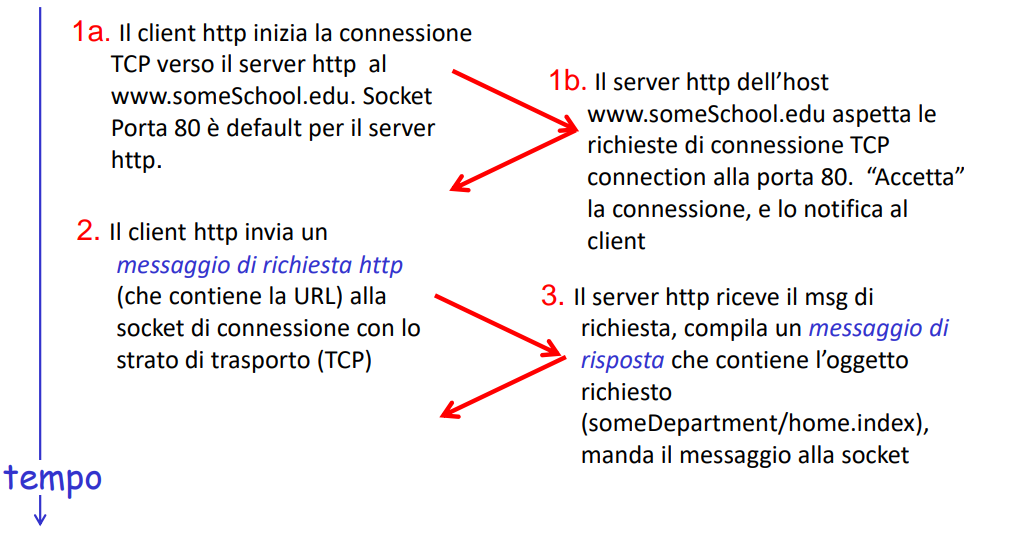
\includegraphics[scale=0.28]{Immagini/Esempio_richiesta_HTTP.png}
    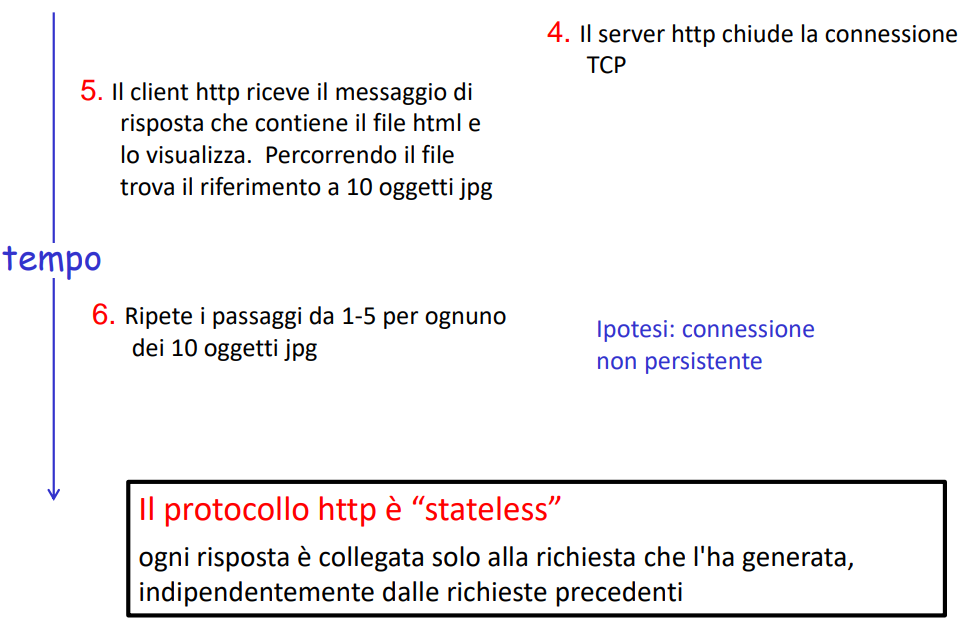
\includegraphics[scale=0.30]{Immagini/Esempio_richiesta_HTTP_2.png}
    \caption{Esempio di interazione con protocollo HTTP.}
\end{figure}

\newpage

L'utilizzo di una connessione persistente non permette di base ad un client di inviare una serie di richieste per ricevere una corrispondente serie di risposte; l'instaurazione di una connessione persistente ha lo scopo principale di migliorare le prestazioni della comunicazione.
\paragraph{Pipelining}Il \textcolor{purple}{Pipelining} è una tecnica di trasmissione delle richieste che consiste nell’invio da parte del client di molteplici richieste senza
aspettare la ricezione di ciascuna risposta. Il server deve inviare le risposte nello stesso ordine in cui sono state ricevute le richieste.
\newline I server web che rispettano HTTP/1.1 devono supportare il pipelining, ma allo stesso tempo pochi browser web supportano questa tecnica. Questo accade perché se una richiesta necessita tempo per essere processata, le risposte alle richieste successive sono bloccate (\textcolor{purple}{Head of Line Blocking}) e in questi casi lo scopo principale di migliorare le prestazioni viene a mancare.

\subsubsection{Formato messaggi HTTP}
Come detto i messaggi HTTP possono essere di tipo richiesta o risposta, la struttura del messaggio è però la medesima:
\begin{itemize}
    \item \textcolor{purple}{Start line}
    \item \textcolor{purple}{Header}
    \item \textcolor{purple}{Body}
\end{itemize}

\paragraph{HTTP request line} Nella start line denominata \textcolor{purple}{Request-Line} per i messaggi di richiesta sono presenti tre campi:
\begin{itemize}
    \item \textcolor{blue}{Method:} operazione che il client richiede al server venga effettuata. I metodi più comuni sono GET, POST, PUT e DELETE;
    \item \textcolor{blue}{Request-URI:} risorsa sulla quale il client vuole venga eseguita l'operazione;
    \item \textcolor{blue}{HTTP-Version:} il mittente indica il formato del messaggio e la sua capacità di comprendere ulteriori comunicazioni HTTP. 
\end{itemize}

\paragraph{HTTP status line} Nella start line denominata \textcolor{purple}{Status-Line} per i messaggi di risposta sono presenti tre campi:
\begin{itemize}
    \item \textcolor{blue}{HTTP-Version}
    \item \textcolor{blue}{Status-Code:} intero a tre cifre che sta ad indicare l'esito della rispostsa (sono definiti dal protocollo).
    \item \textcolor{blue}{Reason-Phrase:} descrizione testuale dello status code (pensata per l’utente umano). 
\end{itemize}

\paragraph{Header}
Gli header sono coppie (nome: valore) che specificano alcuni parametri del messaggio trasmesso o ricevuto. Esistono vari tipi di header:
\begin{itemize}
    \item \textcolor{blue}{General Header:} relativi alla connessione (data, codifica, connessione,...);
    \item \textcolor{blue}{Entity Header:} relativi all’entità trasmessa (content-type, content-length, data di scadenza,...);
    \item \textcolor{blue}{RequestHeader:} relativi al messaggio di richiesta;
    \item \textcolor{blue}{Response Header:} relativi al messaggio di risposta;
\end{itemize}
\begin{mdframed}
    GET http://192.168.11.66/ HTTP/1.1\newline
    host: 192.168.11.66\newline
    Connection: close\newline
    \\
    HTTP/1.1 200 OK\newline
    Date: Sun, 14 May 2000 23:49:39 GMT\newline
    Server: Apache/1.3.9 (Unix) (Red Hat/Linux)\newline
    Last-Modified: Tue, 21 Sep 1999 14:46:36 GMT\newline
    ETag: "f2fc-799-37e79a4c"\newline
    Accept-Ranges: bytes\newline
    Content-Length: 1945\newline
    Connection: close\newline
    Content-Type: text/html\newline
    \\
    $<$!DOCTYPE HTML PUBLIC "-//W3C//DTD HTML 3.2 Final//EN"$>$\newline
    $<$HTML$>$\newline
    $<$HEAD$>$$<$TITLE$>$Test Page for Red Hat Linux's Apache Installation$<$/TITLE$>$$<$/HEAD$>$\newline
    $<$H1 ALIGN="CENTER"$>$It Worked!$<$/H1$>$\newline
    $<$P$>$\newline
    If you can see this, it means that the installation of the $<$AHREF="http://www.apache.org/"$>$Apache$<$/A$>$ software on this $<$ahref="http://www.redhat.com/"$>$Red Hat Linux$<$/a$>$ system was successful. You may now add content to this directory and replace this page.\newline
    $<$/P$>$\newline
    $<$/BODY$>$\newline
    $<$/HTML$>$\newline    
\end{mdframed}

\paragraph{Content Negotation}
Le risorse che un client richiede possono essere disponibili in più rappresentazioni (lingua, formato di dati, dimensione, ecc..). La \textcolor{purple}{Content-Negotiation} è un meccanismo per selezionare la rappresentazione appropriata quando viene servita una richiesta (uso di Request e Entity headers).

\newpage

\subsubsection{Metodi}
\paragraph{OPTIONS} Permette di richiedere al server di fornire le opzioni di comunicazione associate ad un URL o al server stesso (le sue capacità, metodi esposti,...).
\begin{mdframed}
    \textcolor{blue}{OPTIONS http://192.168.11.66/manual/index.html}\newline
    HTTP/1.1\newline
    host: 192.168.11.66\newline
    Connection: close\newline
    \\
    HTTP/1.1 200 OK\newline
    Date: Sun, 14 May 2000 19:52:12 GMT\newline
    Server: Apache/1.3.9 (Unix) (Red Hat/Linux)\newline
    Content-Length: 0\newline
    Allow: GET, HEAD, OPTIONS, TRACE\newline
    Connection: close
\end{mdframed}

\paragraph{GET} Permette di richiedere il trasferimento di una risorsa identificata da una URL o operazioni associate all’URL stessa.
\begin{mdframed}
    \textcolor{blue}{GET http://192.168.11.66 HTTP/1.1}\newline
    host: 192.168.11.66\newline
    Connection: close\newline
    \\
    \textcolor{blue}{HTTP/1.1 200 OK}\newline
    Date: Sun, 14 May 2000 19:57:13 GMT\newline
    Server: Apache/1.3.9 (Unix) (Red Hat/Linux)\newline
    \textcolor{blue}{Last-Modified: Tue, 21 Sep 1999 14:46:36 GMT}\newline
    ETag: "f2fc-799-37e79a4c"\newline
    Accept-Ranges: bytes\newline
    Content-Length: 1945\newline
    Connection: close\newline
    Content-Type: text/html\newline
    $<$!DOCTYPE HTML PUBLIC "-//W3C//DTD HTML 3.2 Final//EN"$>$\newline
    $<$HTML$>$ ...
\end{mdframed}

\paragraph{Conditional GET} Una variante del GET detta GET-Condizionale permette di modificare la risposta del server in base agli header utilizzati (Non modifica il numero totale di messaggi HTTP inviati).
\newpage
\begin{mdframed}
    \textcolor{blue}{GET http://192.168.11.66 HTTP/1.1}\newline
    Host: 192.168.11.66\newline
    \textcolor{blue}{If-Modified-Since: Tue, 21 Sep 1999 14:46:36 GMT}\newline
    \\
    \textcolor{blue}{HTTP/1.1 304 Not Modified}\newline
    Date: Wed, 22 Sep 1999 15:06:36 GMT\newline
    Server: Apache/1.3.9 (Unix) (Red Hat/Linux)\newline
\end{mdframed}

\paragraph{HEAD}
Simile al GET, ma il server non trasferisce il message body nella risposta.
Utile per controllare lo stato dei documenti (validità, modifiche, cache refresh).

\paragraph{POST} Permette al client di inviare informazioni al server, le quali vengono inserite nel body.\newline
\\
Lo standard afferma che:\newline
\emph{Il metodo POST è usato per chiedere che il server accetti l’entità (risorsa)
nel corpo della richiesta come una nuova subordinata della risorsa
identificata dalla Request-URI nella Request-Line.}
\\
\newline
Nella pratica la funzione effettivamente eseguita dal metodo POST è determinata dal server e dipendente tipicamente dalla Request-URI.
\newline
NB: con le API REST vengono rispettate le specifiche HTTP.

\paragraph{PUT} Permette al client di chiedere al server di creare o modificare (se già esistente) una risorsa specificata nell'URI.

\paragraph{DELETE} Permette al client di chiedere al server di cancellare una risorsa identificata dalla Request URI.
\\ \\ NB: I metodi PUT e DELETE sono normalmente non abilitati sui server web pubblici.

\paragraph{Metodi sicuri} Con \textcolor{purple}{metodi sicuri} si fa riferimento a quei metodi che non hanno "effetti collaterali" (per esempio modificare una risorsa). Questi sono: GET, HEAD, OPTIONS e TRACE.

\paragraph{Metodi idempotenti} Con \textcolor{purple}{metodi idempotenti} si fa riferimento a qeui metodi che presentano la proprietà per la quale $N>0$ richieste identiche tra loro hanno lo stesso effetto di una singola richiesta. Questi metodi sono: GET, HEAD, PUT, DELETE, OPTIONS, TRACE.

\subsubsection{Caching e Cookie}
\paragraph{Web Caching} Tecnica che ha lo scopo principale di soddisfare richieste del client senza contattare i server. Consiste nel memorizzare copie temporanee di risorse Web e servirle al client per ridurre l’uso di risorse e diminuire tempo di risposta. I due principali approcci sono:
\begin{itemize}
    \item \textcolor{purple}{User Agent Cache:} il browser mantiene una copia delle risorse visitate dall'utente per quando queste verranno nuovamente visitate.
    \item \textcolor{purple}{Proxy Cache:} server proxy dedicati si intrappongono tra il client e il server. Quando un client esegue una richiesta questa passa per il server proxy e se è già stata memorizzata viene restituita al client; altrimenti il proxy si preoccupa di inoltrare la richiesta al server di competenza e una volta ricevuta la risposta la memorizza e la inoltra al client.
\end{itemize}

\paragraph{Cookie} I \textcolor{purple}{Cookie} sono un meccanismo con il quale è possibile memorizzare delle informazioni su un certo client.
Come detto HTTP è un protocollo state-less perciò un server non ha modo di tenere traccia dei client (anche perché questi di norma non hanno un ip statico).
La prima volta che un client invia un messaggio HTTP ad un server, questo lo "obbliga" a memorizzare un'insieme di informazioni che verranno utilizzate nelle successive comunicazioni.
\newline Gli utilizzi principali dei cookie sono: autenticazione, memorizzazione dati form e in generale creare sessioni su un protocollo state-less.

\begin{figure}[h]
    \centering
    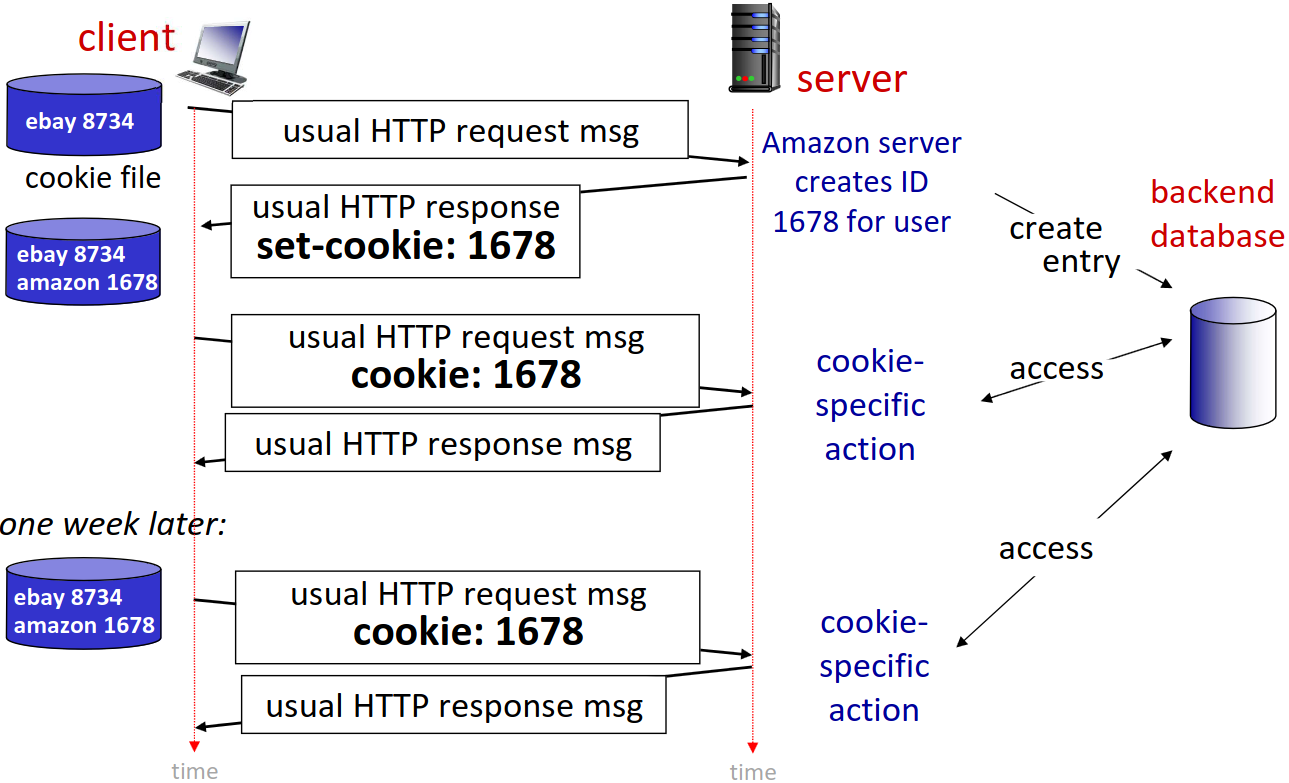
\includegraphics[scale=0.25]{Immagini/Cookie.png}
    \caption{Esempio di interazione con protocollo HTTP e utilizzo di cookie}
\end{figure}
\newpage
\subsection{TELNET} Il protocollo \textbf{\textcolor{purple}{TErminL NETwork}} ha lo scopo principale di permettere l'uso interattivo di macchine remote. Funzionamento:
\begin{enumerate}
    \item la macchina locale stabilisce una connessione con un server login remoto;
    \item tutte le battute dei tasti della macchina locale vengono inviate alla macchina remota, la quale esegue i comandi come se fossero stati battuti sulla macchina stessa.
    \item l'output viene inoltrato dalla macchina remota alla macchina locale;
\end{enumerate}
Per poter garantire questo funzionamento il modello di telnet include:
\begin{itemize}
    \item Un \textcolor{blue}{programma server} che accetta le richieste;
    \item Un \textcolor{blue}{programma client} che effettua le richieste e interagisce direttamente con l'utente;
\end{itemize}
La connessione viene realizzata mediante il protocollo TCP sulla porta 23.

\begin{figure}[h]
    \centering
    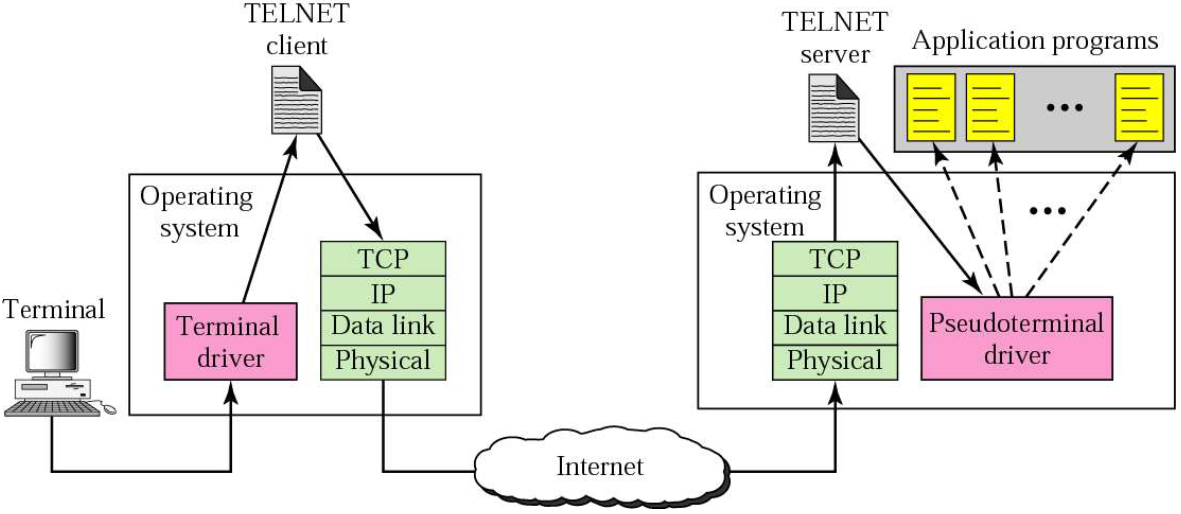
\includegraphics[scale=0.27]{Immagini/Schema_Telnet.png}
    \caption{Esempio di interazione con protocollo TELNET}
\end{figure}

\newblock

\paragraph{NVT} Telnet deve poter operare con il numero massimo di sistemi e quindi gestire dettagli di sistemi operativi eterogenei (i quali possono differire per numerosi aspetti).
Per risolvere il problema client e server devono eseguire un \textcolor{purple}{Network Virtual Terminal} il quale effettua la codifica dei caratteri del sistema locale nel set di caratteri e comandi specifici della NVT.
\begin{figure}[h]
    \centering
    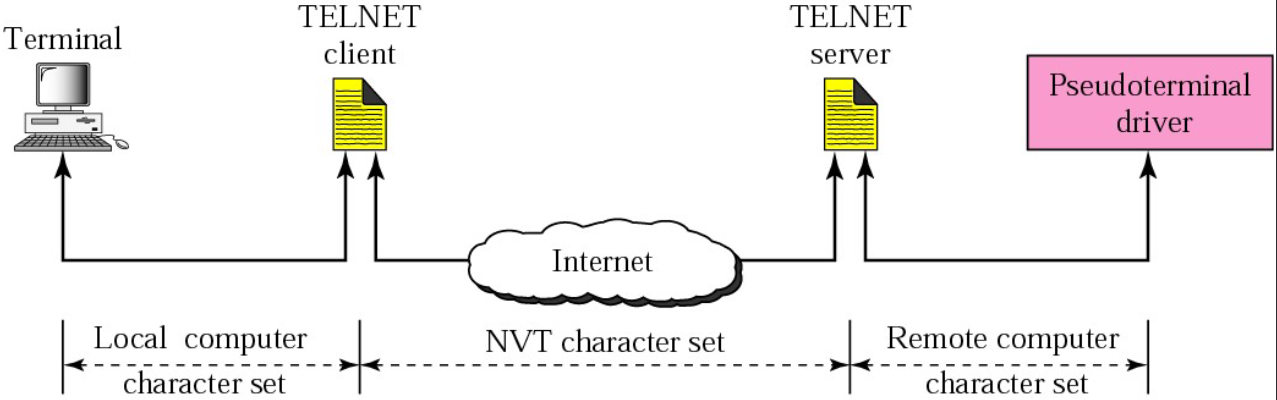
\includegraphics[scale=0.27]{Immagini/Telnet_NVT.png}
    \caption{Esempio di interazione con protocollo TELNET e NVT}
\end{figure}

Gli NVT si scambiano dati in formato 7-bit US-ASCII. Ogni carattere è inviato come un ottetto con il primo bit settato a zero.
I byte con il bit più significativo a 1 vengono usati per le sequenze di comandi e vengono preceduti da un ottetto speciale detto IAC (Interpret as Command).
\\ \\ I messaggi di controllo iniziali sono usati per scambiare informazioni sulle caratteristiche degli host (\textcolor{purple}{Telnet option negotiation}).

\paragraph{Sicurezza} Telnet non è un protocollo sicuro inquanto tutte le comunicazioni tra macchina locale e remota avvengono in chiaro.

\subsection{Email}
\paragraph*{Posta Elettronica} La posta elettronica è uno dei primi servizi applicativi di internet che consiste nel trasferimento di un messaggio tra uno user mittente ed uno user destinatario.
Il servizio di posta elettronica si basa su componenti intermedi per trasferire i messaggi (disaccoppiando mittente e destinatario) per risolvere il problema di disponibilità del destinatario:
\begin{itemize}
    \item computer spento;
    \item utente impegnato.
\end{itemize}
I componenti sono:
\begin{itemize}
    \item \textcolor{purple}{User Agent}, per la composizione, editing, lettura di messaggi di posta (Outlook, Eudora,...);
    \item \textcolor{purple}{Mail Server}, il quale presenta:
        \begin{itemize}
            \item \textcolor{blue}{Mail Box}, dove sono archiviati messaggi in ingresso che devono ancora essere letti dall'utente;
            \item una coda dei messaggi in uscita che devono essere ancora inviati.
        \end{itemize}
    \item \textcolor{purple}{protocollo SMTP}, che permette il dialogo tra i Mail Server:
        \begin{itemize}
            \item \textcolor{blue}{client}, mail server che invia i messaggi;
            \item \textcolor{blue}{server}, mail server che riceve i messaggi.
        \end{itemize}
\end{itemize}

\paragraph{Indirizzo Mail}
Un destinatario è identificato da un indirizzo email nella forma:
\begin{center}
    local-part @ domain-name
\end{center}
\begin{itemize}
    \item \textcolor{blue}{domain-name}, specifica un mail server. Determina il nome di dominio di una destinazione a cui la mail dovrebbe essere recapitata.
    \item \textcolor{blue}{local-part}, pecifica la cassetta di posta nel mail server. Spesso è identica al nome di login o al nome completo dell’utente.
\end{itemize}

\paragraph{Spooling} I server si posta elettronica addottano un tecnica denominata \textcolor{purple}{spooling}:
\begin{enumerate}
    \item L'utente invia un messaggio e il server ne pone una copia in un'area di memoria denominata \textcolor{blue}{spool} (o anche area di accodamento della posta) insieme a:
        \begin{itemize}
            \item id mittente;
            \item id destinatario;
            \item id macchina destinazione;
            \item tempo di deposito.
        \end{itemize}
    \item Il sistema (\textcolor{blue}{client}) avvia il trasferimento alla macchina remota stabilendo con essa una connessione TCP:
        \begin{itemize}
            \item se la connessione viene aperta e il trasferimento va a buon fine allora il client cancella la copia locale della mail;
            \item altrimenti, il client scandisce periodicamente l'area di spool e tenta il trasferimento dei messaggi non consegnati. Oltre un certo intervallo di tempo (definito dall’amministratore del server) se il messaggio non è stato consegnato, viene inviata una notifica all’utente mittente.
        \end{itemize}
\end{enumerate}

\paragraph{Alias}
\begin{definition}
    Un \textcolor{purple}{alias} è una cassetta postale virtuale che serve a ridistribuire i messaggi verso uno o più indirizzi di posta elettronica personali.
\end{definition}

Esistono due tipologie di alias:
\begin{itemize}
    \item \textcolor{purple}{molti-uno:} il sistema di alias permette ad un singolo utente di avere identificatori di mail multipli, assegnando un set di identificatori ad una singola persona;
    \item \textcolor{purple}{uno-molti:} il sistema permette di associare un gruppo di destinatari ad un singolo identificatore.
\end{itemize}

\subsubsection{SMTP}
\textbf{\textcolor{purple}{Simple Mail Transfer Protocol}} ha come obiettivo principale il trasferimento affidabile ed efficiente di mail.
Le principali caratteristiche sono:
\begin{itemize}
    \item indipendenza dal sistema di trasmissione usato, SMTP richiede solo il trasferimento di stream di byte ordinato e affidabile.
    \item la capacità di trasportare mail attraverso più reti. Un messaggio di mail può passare attraverso server intermedi nel percorso da mittente a destinatario finale.
\end{itemize}
SMTP è detto protocollo di tipo \textcolor{purple}{push}.

\paragraph{Modello di SMTP}
Quando un client SMTP vuole trasferire un messaggio, stabilisce un canale di trasmissione bidirezionale con un server SMTP. 
La responsabilità di un client è di trasferire la mail a un server SMTP, o comunicare un eventuale insuccesso (scambio formale di responsabilità).
Un client SMTP determina l’indirizzo di un host appropriato che ospita un server SMTP risolvendo il nome della destinazione in un indirizzo del mail server destinazione.
\\Possibile problemi possono essere:
\begin{itemize}
    \item connessione con mailserver del mittente (server inesistente o irraggiungibile);
    \item connessione con mailserver destinatario (server inesistente o irraggiungibile);
    \item inserimento in mailbox destinatario (user unknown, mailbox full).
\end{itemize}
In \underline{tutti} questi casi il mittente riceve una notficata.

\paragraph{Protocollo}
Il trasferimento via SMTP avviene in tre fasi:
\begin{enumerate}
    \item \textcolor{purple}{Handshaking:} Una volta stabilita la connessione TCP il clinet attende che il server invii \textbf{220 READY FOR MAIL}. A questo punto il client invia il comando \textbf{HELO} e il server risponde identificandosi;
    \item \textcolor{purple}{Trasferimento del messaggio:} Inizia la trasmissione del messaggio, il quale è suddiviso in:
        \begin{itemize}
            \item \textcolor{blue}{Header:} che contiene informazioni sul mittente, destinatario e oggetto del messaggio;
            \item \textcolor{blue}{Body:} il contenuto del messaggio vero e proprio, codificato in 7-bit US-ASCII
        \end{itemize}
    \item \textcolor{purple}{Chiusura della connessione.}
\end{enumerate}

\begin{figure}[h]
    \centering
    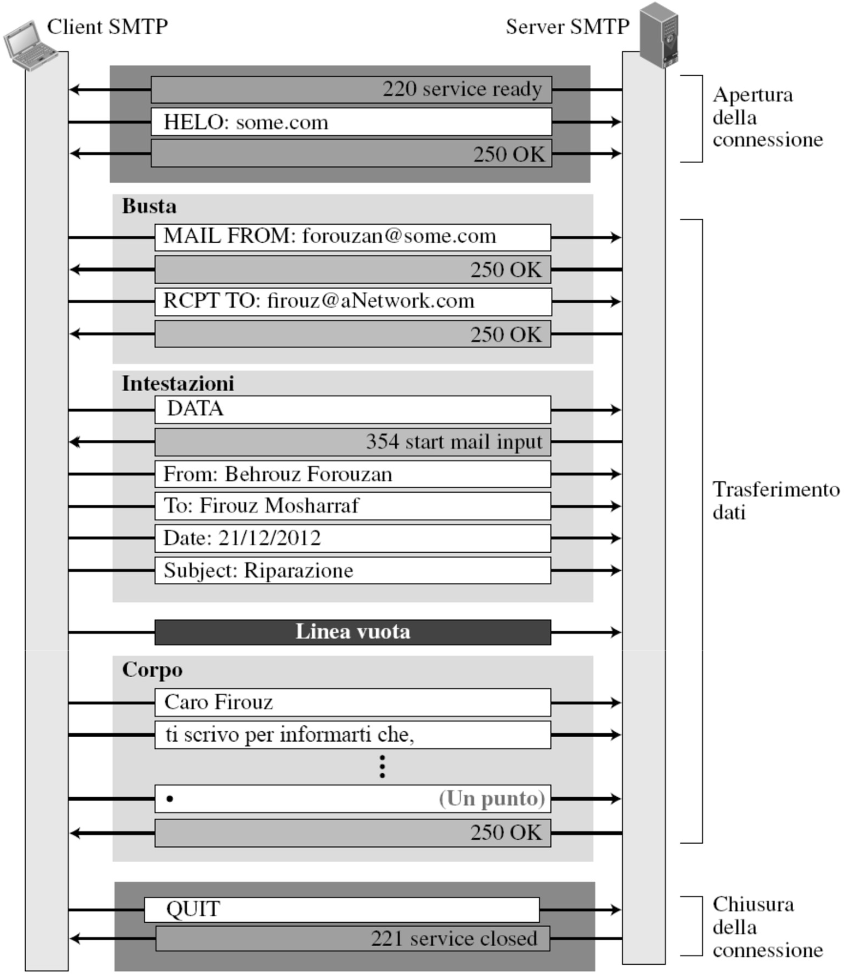
\includegraphics[scale=0.30]{Immagini/Comunicazione_SMTP.png}
    \caption{Esempio di interazione con protocollo SMTP}
\end{figure}

\newblock
La fine di un messaggio in SMTP è identificata dalla stringa \textbf{$<$CRLF$>$.$<$CRLF$>$} (un punto).
\newpage
\subsubsection{Estensioni multimediali} 
La codifica 7-bit US-ASCII è molto restrittiva, infatti non supporta: accenti, lingue non latine, lingue senza alfabeti e contenuti multimediali come audio o video.
\\Per risolvere questo probelma senza dover in alcun modo apportare modifiche ai Mail Server già esistenti, si è deciso di definire regole di codifica (\textcolor{purple}{encoding}) per il trasferimento di testo non ASCII. (Necessario invece aggiornare o cambiare User Agent)

\paragraph{MIME}
\textcolor{purple}{Multipurpose Internet Mail Extension} è uno standard di Internet che permette di estendere il formato di e-mail per suppportare:
\begin{itemize}
    \item esto in set di caratteri diversi da US-ASCII;
    \item allegati in formato non testuale;
    \item corpo del messaggio con più parti;
    \item header in set di caratteri non-ASCII.
\end{itemize}
MIME definisce un insieme di metodi per rappresentare dati binari in formato ASCII.
\\MIME fornisce vari schemi di transfer encoding, tra cui:
\begin{itemize}
    \item \textcolor{purple}{Base64 Encoding:} gruppi di 24 bit sono divisi in 4 unità da 6 bit e ciascuna unità viene inviata come un carattere ASCII;
    \item \textcolor{purple}{Quoted-printable encoding:} per messaggi testuali con pochi caratteri non-ASCII, più efficiente.
\end{itemize}

L'utlizzo di questo standard per messaggi inviati con SMTP richiede l'utilizzo di ulteriori righe di intestazione per specificare: la versione MIME, il tipo di contenuto, ...

\subsubsection{Accesso alla posta}
Abbiamo visto come SMTP sia un protocollo di tipo push con il quale è possibile inviare un messaggio di posta elettronica fino al Mail server di destinazione. 
Per recuperare il messaggio però abbiamo bisogno di un protocollo di tipo \textcolor{purple}{pull}, come per esempio:
\begin{itemize}
    \item \textbf{\textcolor{purple}{POP3}}
    \item \textbf{\textcolor{purple}{IMAP}}
    \item \textbf{\textcolor{purple}{HTTP:}} Hotmail , Yahoo! Mail, Gmail, ...
\end{itemize}

\paragraph{POP3} Lo User Agent del destinatario apre una connessione TCP, sulla porta 110, con il Mail Server e iniziano così le tre fasi per il recupro dei messaggi:
\begin{itemize}
    \item \textcolor{purple}{Autorizzazione:} Il client esegue l'accesso specificando username e password;
    \item \textcolor{purple}{Scambio:} Il client con una serie di comandi visualizza i messaggi (\textcolor{blue}{list}), li preleva (\textcolor{blue}{retr}), marca i messaggi da eliminare sul server (\textcolor{blue}{dele}) e chiude la sessione (\textcolor{blue}{quit});
    \item \textcolor{purple}{Aggiornamento: } Il server, dopo aver ricevuto il comado quit, cancella i messaggi marcati per la rimozione.
\end{itemize}

NB: POP3 non mantiene informazioni di stato tra sessioni

\paragraph{IMAP}
IMAP è un altro protocollo di tipo pull per il recupero di messaggi dai Mail server. 
Presenta più feature di POP3 (per questo è anche più complesso) come la manipolazione dei messaggi memorizzati sul server e comandi per estrarre solo alcune componenti dei messaggi.

\subsection{DNS}
Agli albori di Internet l'associazione tra nomi logici ed indirizzi IP era statica. 
Tutte le associazioni erano contenute in un unico file, detto \textcolor{purple}{host file}, e periodicamente gli host prelevavano una versione aggiornata del file, \textcolor{purple}{master host file}, da un server ufficiale.
Date le dimensioni attuali di Internet, questo approcio è impraticabile per motivi di scalabilità.
\\
\\Il \textbf{\textcolor{purple}{DNS}} (Domain Name System) ha l'obiettivo principale di fornire un meccanismo per:
\begin{itemize}
    \item specificare la sintassi dei nomi e le regole per gestirli;
    \item consentire la conversione dei nomi in indirizzi e viceversa.
\end{itemize}
Esso è costituito essenzialmente da:
\begin{itemize}
    \item uno \textcolor{purple}{schema di assegnazione dei nomi} gerarchico e basato su domini;
    \item un \textcolor{purple}{database distribuito} contenente i nomi e le corrispondenze con gli indirizzi IP impolementato con una gerarchia di name server;
    \item un \textcolor{purple}{protocollo} per la distribuzione delle informazioni sui nomi tra name server basato su:
        \begin{itemize}
            \item paradigma client/server, in cui i server comunicano tra loro per \textcolor{blue}{risolvere} nomi (traduzione nome/indirizzo);
            \item protocolli di trasporto UDP e TCP.
        \end{itemize}
\end{itemize}

\paragraph{Servizi} I servizi offerti dal DNS sono:
\begin{itemize}
    \item \textbf{\textcolor{purple}{Host aliasing:}} Traduzione dei nomi in nome canonico/indirizo IP (un host può avere più nomi dei quali, uno è detto canonico mentre gli altri sinonimi); 
    \item \textbf{\textcolor{purple}{Mail server aliasing:}} analogo all'host aliasing ma viene distinto perché potrebbero esistere nomi (sinonimi) identitici tra web server e mail server;
    \item \textbf{\textcolor{purple}{Distribuzione di carico:}} Ad un nome canonico potrebbero essere associati più indirizzi IP (server replicati) ed in questo caso il DNS restituisce la lista di indirizzi IP variandone l'ordinamento ad ogni risposta.
\end{itemize}

\begin{figure}[h]
    \centering
    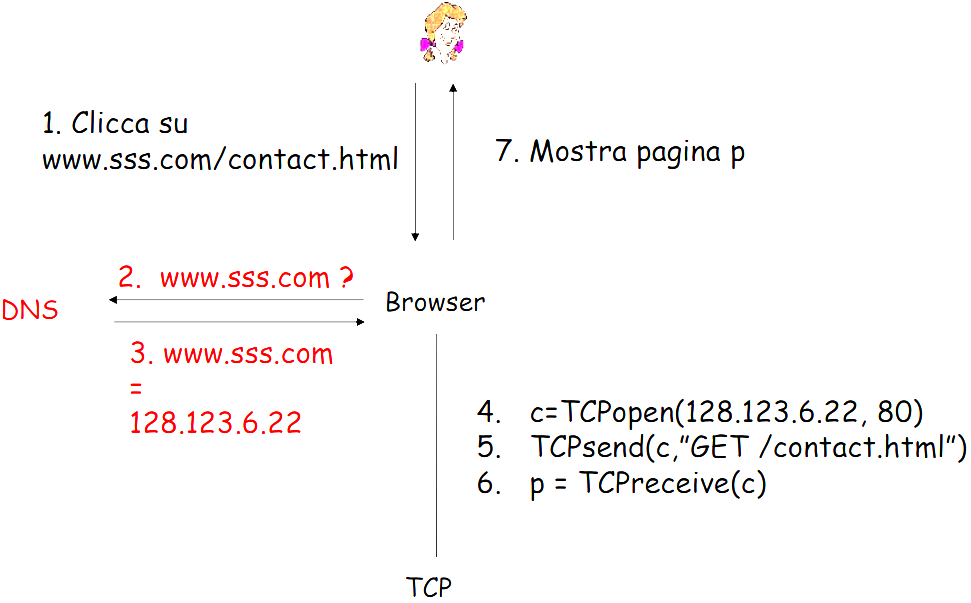
\includegraphics[scale=0.45]{Immagini/PosizionamentoDNS.png}
    \caption{Il DNS si frappone tra client e server (Non interagisce mai direttamente con l'utente).}
\end{figure}

\subsubsection{Spazio dei nomi}
\paragraph{Struttura dei nomi} I nomi devo permettere di identificare in mood univoco un host. Questi presentano un struttura gerarchica, infatti un nome è costituito da diverse parti (es. \textcolor{green}{lab3}.\textcolor{blue}{di}.\textcolor{red}{unipi}.\textcolor{violet}{it}).
\\L'assegnazione dei nomi è delegabile, infatti il sistema è in buona parte decentralizzato. La delega avviene a favore dell'autorità per l’assegnazione delle varie parti dello spazio dei nomi.
\\In questo modo si distribuisce la responsabilità della conversione tra nomi e indrizzi.
\paragraph{Nomi di dominio} I nomi hanno una struttura ad albero con un numero di livelli variabile ed ogni nodo è identificato da un'etichetta (di massimo 63 caratteri) ed ha un nome di dominio dato da una sequenza di etichette separate da punto. Alla radice è associata un'etichetta vuota.
\begin{definition}[Dominio] 
    Con \textcolor{purple}{Dominio} si fa riferimento ad un sottoalbero nello spazio dei nomi di dominio che viene identificato dal nome di dominio del nodo radice del sotto albero.
\end{definition}

\begin{figure}[h]
    \centering
    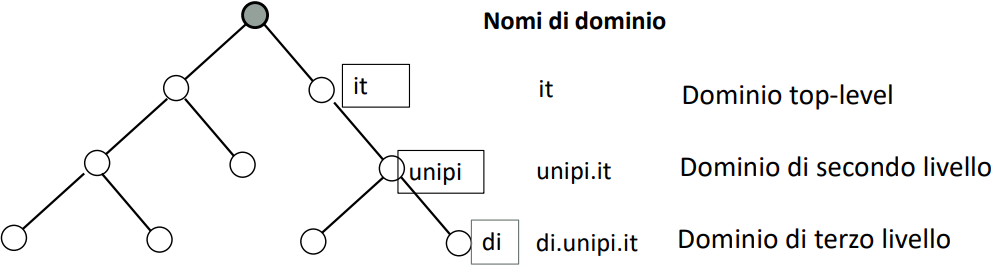
\includegraphics[scale=0.45]{Immagini/StrutturaNomiDiDominio.png}
    \caption{Struttura Domini}
\end{figure}

Un dominio può essere suddiviso in ulteriroi domini detti sottodomini.
In Internet i nomi gerarchici delle macchine sono assegnati in base alla struttura delle organizzazioni che ottengono l'autorità su porzioni dello spazio dei nomi.
\\In questo modo è sempre garantità l'univocità dei nomi.

\subsubsection{Gerarchia dei NameServer}
Per ogni dominio non è presente un unico NameServer ma un insieme di essi, per migliorare le prestazioni e per motivi di sicurezza.
\begin{definition}[Zona]
    Una \textcolor{purple}{Zona} è una porzione dello spazio dei nomi di dominio che è gestita da una specifica amministrazione.
\end{definition} 
NB: Zona e Dominio non necessariamente conicidono.
\\\\Ogni server immagazzina le informazioni relative alla propria zona inclusi i riferimenti ai name server dei domini di livello inferiore.

\paragraph{Gerarchia} La gerarchia è così composta:
\begin{itemize}
    \item \textbf{\textcolor{purple}{Server Radice:}} responsabile dei record della zona radice, riconosce tutti i domini di massimo livello (TLD - Top Level Domain) e restituisce infomrazioni su essi;
    \item \textbf{\textcolor{purple}{Server Top-Level Domain:}} mantiene le informazioni dei nomi di dominio che appartengono al suo TLD e restituisce informazioni sui nameserver di competenza dei sottodomini.
    \item \textbf{\textcolor{purple}{Authoritative Name Server:}} autorità di una certa zona che memorizza nome e indirizzo IP di un insieme di host. Per ogni zona possono essere presenti server di competenza primari e secondari. I server di competenza primari mantengono il file di zona (file contenente le associazioni nome/indirizzo più aggiornate) mentre i server di competenza secondari ricevono il file di zona e offorno il servizio di risoluzione.
\end{itemize}

\paragraph{Local Name Server}


% da finire quando lo farà a lezione
% \subsection{FTP}
% Il protocollo \textbf{\textcolor{purple}{File Transer Protocol}} è il protocollo standard per il trasferimento file in reti TCP/IP. Offre inoltre altre funzionalità, oltre al semplice trasferimento file, come l'accesso interattivo all'albero delle directory del FileSystem remoto e un accesso con autenticazione.

% \paragraph{Modello FTP} FTP mette a disposizione due differenti tipologie di connessione tra client e server:
% \begin{itemize}
%     \item \textcolor{blue}{Control connection:} connessione dedicata allo scambio di comandi e risposte (come Telnet);
%     \item \textcolor{blue}{Data connection:} connessione su cui i dati sono trasferiti con modi e tipi specificati. I dati trasferiti possono essere parte di un file, un file o un set di file.
% \end{itemize}

% FTP è un protocollo \textcolor{purple}{statefull}, infatti il server deve tenere traccia dello stato dell'utente (connessione di controllo associata ad un account, directory attuale,...).
% \paragraph{Connessione di Controllo} Il clinet FTP contatta il server FTP sulla porta 21 e, una volta ottentuta l'autorizzazione dal server, utilizzerà questa connessione per scambiare comandi. 
% La comunicazione sulla connessione di controllo avviene per mezzo di caratteri con una codifica standard NVT ASCII, sia per i comandi che per le risposte (Telnet).
% \\Questa connessione è di tipo \textcolor{purple}{persistente}.
% \\Quando il client attiva la connessione di controllo con il server, usa un numero di porta assegnato localmente in modo casuale e FTP usa la connessione di controllo per permettere a client e server di coordinare l’uso delle porte assegnate dinamicamente per il trasferimento dati.

% \paragraph{Connessione Dati} 